\documentclass[12pt,a4paper]{article}

\usepackage[margin=0.7in]{geometry}
\usepackage{amssymb, amsthm, amsmath, amsfonts}
\usepackage{array, xcolor, enumitem, graphicx}
\usepackage{cancel}

\usepackage[czech]{babel}
\usepackage[utf8]{inputenc}
\usepackage[unicode]{hyperref}
\usepackage[useregional]{datetime2}

\hypersetup{
    colorlinks=true,
    linkcolor=black,
    urlcolor=blue,
    pdftitle={Specifikace},
}

% tahak - prikazy %
% \includegraphics{obrazek.png}         % import konkretniho obrazku
% a~b                                   % mezera mezi pismeny 'a' a 'b'
% a \quad b                             % velka mezera mezi pismeny 'a' a 'b'
% \sim                                  % ~
% \Longleftarrow                        % <==


% zkratky %

\newcommand{\hr}{{\begin{center}\par\rule{\textwidth}{0.5pt} \end{center}}}
\newcommand\makesmall{\fontsize{8pt}{11pt}\selectfont}

\renewcommand*{\figurename}{\makesmall Obr.}

% hlavicka
\setlength{\parindent}{0em}

\title{Specifikace softwarového díla\\ \&\\ Časový plán implementace pro\\ \LARGE{Mobilní aplikace sloužící k ovládání ToF kamer}}
\date{31. května 2024}
\author{\sc Karel Velička}

\graphicspath{ {img/} }             % obrazky ulozeny ve slozce img/

\begin{document}

%\maketitle
\thispagestyle{empty} 	%tato stránka se nebude číslovat
\begin{center}
    {\LARGE Specifikace softwarového díla\\ \&\\ Časový plán implementace pro\\[5mm] Mobilní aplikace sloužící k ovládání ToF kamer}
    \line(1,0){400}\\ [10mm]
    
    {\large Projekt se zaměřuje na vývoj mobilní aplikace pro ovládání ToF kamer přes Raspberry Pi.
    Aplikace umožní uživateli komunikovat přes Bluetooth a na dálku tak nahrávat a přehrávat zaznamenaný obsah.} % lze procentem zapoznámkovat
    
    \vfill    


    Verze: 1.0.1 \\[10mm]
    \sc Karel Velička\\ [10mm]
    31. května 2024
    
    ~ \\ [1cm]
    \end{center}

% podnadpis + obsah 
\begin{center}
    
\end{center}

\begin{center}
   
\end{center}

\newpage
\tableofcontents

\pagenumbering{arabic}

\newpage

% obsah dokumentu

\section{Základní informace}

\subsection{Popis a zaměření softwarového díla}

ToF kamera je zařízení, které využívá technologii Time-of-Flight k měření vzdálenosti. 
Kamera vysílá infračervené světlo, které se odráží od objektů a vrací zpět k senzoru. 
Na základě času, který světlu trvá cesta tam a zpět, kamera vypočítá vzdálenost k jednotlivým objektům, čímž umožňuje přesnou detekci pohybu a tvarů v prostoru.

$ $

Existují již podobné projekty, které se zaměřily na zobrazování záznamu z ToF kamer, příkladem může být třeba \href{https://github.com/ArduCAM/Arducam_tof_camera}{ArduCAM}, nebo \href{https://github.com/espros/epc-tofcam-toolkit}{espros}.
Nicméně žádná implementace prozatím není v jazyce Java a žádná implementace nezajišťuje přenos do mobilního telefonu skrz Bluetooth.

$ $

Tento projekt se tedy zaměřuje na vývoj mobilní aplikace v systému Android, která umožní uživateli komunikovat přes Bluetooth a na dálku tak nahrávat a přehrávat zaznamenaný obsah z kamery.

\subsection{Použité technologie}

V projektu jsou použita zařízení \textit{Nucleo board STM32F401} spolu s kamerou \textit{VL53L5 ToF} a \textit{Raspberry Pi 5}.

Jinak je, pro tvorbu Android aplikace, využito \href{https://developer.android.com/studio/releases/past-releases/as-flamingo-release-notes}{Android Studio Flamingo} a obecně programovací jazyk Java 21 spolu s knihovnami: \begin{itemize}
	\item \href{https://mvnrepository.com/artifact/org.json/json}{JSON In Java} - knihovna usnadňující práci s `.json` soubory
	\item \href{https://mvnrepository.com/artifact/com.fazecast/jSerialComm}{JSerialComm} - knihovna usnadňující práci s porty (připojená zařízení přes USB)
\end{itemize}

\subsection{Konvence tohoto dokumentu}
Odkazy na webové stránky jsou uváděny modrou barvou.
Raspberry Pi bude někdy zkracováno na RPi

\subsection{Odkazy (Reference)}

\begin{itemize}\setlength\itemsep{0em}
	\item Webová stránka s Nucelo board specifikací: \begin{itemize}\setlength\itemsep{0em}
		\item {\footnotesize \href{https://www.st.com/en/evaluation-tools/stm32-nucleo-boards.html}{https://www.st.com/en/evaluation-tools/stm32-nucleo-boards.html}, STMicroelectronics, 2024}
	\end{itemize}
	\item Webová stránka s ToF specifikací: \begin{itemize}\setlength\itemsep{0em}
		\item {\footnotesize \href{https://www.st.com/en/imaging-and-photonics-solutions/vl53l5cx.html}{https://www.st.com/en/imaging-and-photonics-solutions/vl53l5cx.html}, STMicroelectronics, 2024}
	\end{itemize}
\end{itemize}

\newpage
\section{Stručný popis softwarového díla}

\subsection{Důvod vzniku softwarového díla a jeho základní části a cíle řešení}

Důvodem vzniku, jak již bylo popsáno v sekci výše, je neexistence mobilní aplikace komunikující s kamerou ToF.

Projekt je obecně rozdělen do dvou částí, ačkoliv je hlavním ovládacím zařízením právě telefon.
\begin{enumerate}
	\item Získávání informací z ToF kamery. To zajišťuje samostatný skript, který zároveň spouští Bluetooth server a čeká na připojení klienta (mobil).
	\item Mobilní aplikace sloužící jako Bluetooth klient a umožňující nastavit, nahrát  přehrát video záznam.
\end{enumerate}

\subsection{Hlavní funkce}
\begin{itemize}
	\item Připojení přes bluetooth: RaspberryPi $ \rightleftarrows $ Mobilní telefon.
	\item Přehrání video záznamu z JSON souboru.
	\item Nahrání a uložení videa do JSON souboru.
	\item Drobnosti navíc pro zpříjemnění přehrávání - změna FPS, vzdálenost, otáčení kolem osy.
\end{itemize}

\subsection{Motivační příklad užití}

Uživatel spustí na Raspberry Pi (připojené k Nucleo board + ToF) tento program.
Tím se vytvoří Bluetooth server a čeká na připojení klienta.

Uživatel zároveň spustí Mobilní aplikaci, připojí se k Raspberry Pi, vybere si v nastavení vše co požaduje, začne nahrávat.
Následně si přehraje video záznam.

\subsection{Prostředí aplikace}
	Program pro Raspberry Pi bude konzolová Java aplikace fungující také na běžných Linuxových distribucích.
	
	Aplikace pro mobilní telefon bude spustitelná pouze na zařízeních Android 5.0 Lollipop a novějších a bude ovladatelná skrz běžné (defaultní) grafické rozhraní.
\subsection{Omezení díla}

Pro účely práce bude odladěn pouze program pro Raspberry Pi (respektive Linuxová zařízení).

\section{Vnější rozhraní}

\subsection{Uživatelské rozhraní, vstupy a výstupy}
Mobilní aplikace od uživatele dostává veškeré pokyny, které má v nabídce. Umožní se připojit přes Bluetooth, nastavit konfigurační soubor, začít nahrávat a následně spouštět video.


Z hlediska RPi programu je vstupem vždy požadavek získaný od klienta přes Bluetooth.
Požadavek bude ve smyslu "start record", "stop record", "send video", "capture config".
Výstupem pak bude právě nahrané video v JSON formátu. 
Jinak uživatel s tímto programem nijak jinak, než že jej spustí, nekomunikuje.


\subsection{Rozhraní s hardware}

RPi komunikuje s ToF kamerou prostřednictvím micro USB kabelu. Komunikaci nám usnadňuje knihovna \textit{jSerialComm}.

\subsection{Rozhraní se software}

Veškeré \textit{Fragmenty} mobilních rozhraní komunikují s kódem za pomoci \texttt{binding} a \texttt{CreateView}.

Přes Bluetooth se přenese JSON soubor s obsahem videa. JSON soubor se parsuje za pomoci knihovny \textit{JSON In Java}.


\subsection{Komunikační rozhraní}

Komunikace mezi Serverem (RPi) a klientem (Mobil) probíhá prostřednictvím otevřeného standardu Bluetooth verze 5.0 (respektive nižší, pokud Android telefon nepodporuje 5.0).

RPi vytvoří server a čeká na připojení klienta. Android vytvoří požadavek na spárování a následně začne komunikace.

Odesílají se bloky dat v podobě \textit{(hlavička, data)}, kde \textit{hlavička} obsahuje typ požadavku/ zprávy.

\section{Detailní popis funkcionality}

\subsection{Spuštění serveru na RPi}
Uživatel připojí Nucleo board (spolu s ToF) k Raspberry Pi.
Na RPi se spustí program příkazem \texttt{java -jar btof.jar} .
Tím se automaticky vytvoří Bluetooth server a nastane čekání na připojení klienta.

\subsection{Bluetooth připojení}
Uživatel spustí mobilní aplikaci, přejde na \textit{"Bluetooth připojení"}, stiskne \textit{"vyhledat"} a vybere RPi server. (Pokud se zařízení nezobrazí, může stisknout \textit{"refresh"}). Tím je připojen k RPi a tedy i k ToF kameře.

\subsection{Nastavení}
Uživatel může v nastavení nastavit specifikaci pro přehrávání videa.
\textit{Rotace} otočí video přehrávač o $ \{0, 90, 180, 270\}$ stupňů. \textit{FPS} nastaví počet snímků za sekundu (defaultně nastaveno na 10).

Dále je možné nastavit \textit{Detekovaný cíl, Vzdálenost} a \textit{Statistiku}, což jsou textové údaje, které se zobrazí na jednotlivých čtverečcích videa.

\subsection{Přehrávač}
Uživatel může přehrát či pozastavit video. Bude zároveň obsahovat tlačítko "nahrát", které nahraje záznam z kamery.

\newpage
\section{Obrazovky}

\subsection{Mobilní aplikace - Nastavení, Přehrávač, Bluetooth}

\begin{figure}[h]
	\centering
	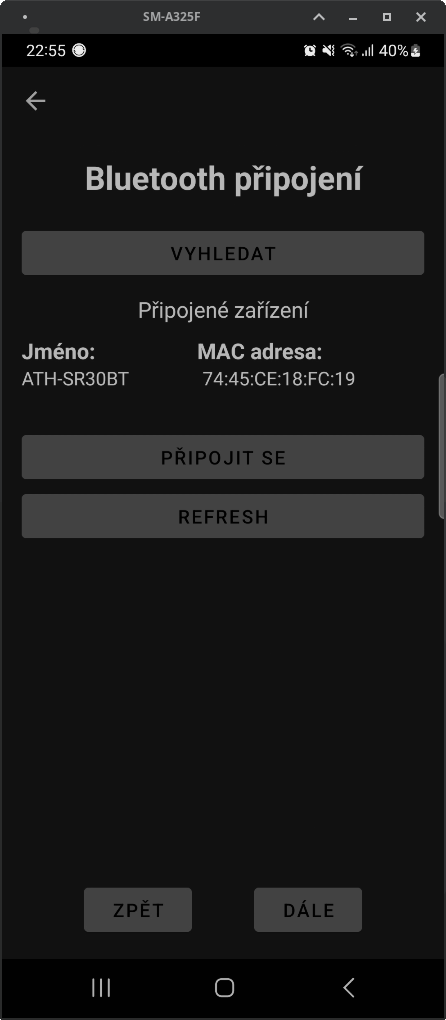
\includegraphics[width=.25\textwidth]{RocnikovyProjekt/bluetooth.png} \qquad
	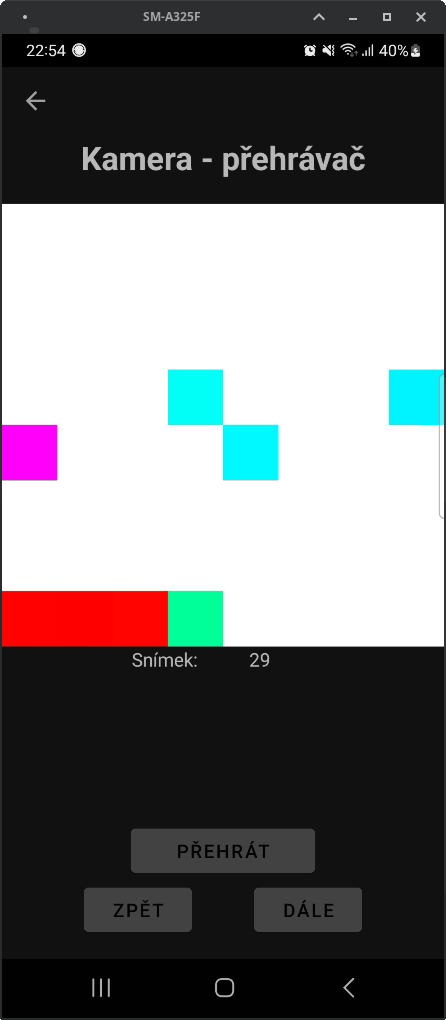
\includegraphics[width=.25\textwidth]{RocnikovyProjekt/camera.png}\qquad
	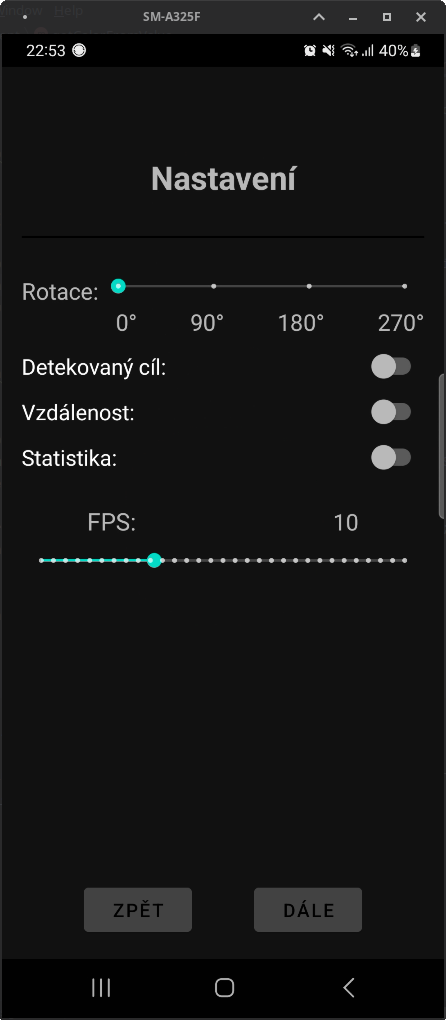
\includegraphics[width=.25\textwidth]{RocnikovyProjekt/nastaveni.png}
	\caption{Jednotlivé náhledy Fragmentů z mobilní aplikace.}
\end{figure}

\section{Time-line \& Milestones}

\begin{center}
	\begin{tabular}{|p{2.5cm} | p{8cm} | p{5cm} |} 
		\hline
		\textbf{Datum} & \textbf{Milník} & \textbf{Způsob prezentace} \\ [0.5ex] 
		\hline
		31. 05. 2024 & Finální verze této specifikace & Existující dokument\\  [0.5ex] 
		\hline
		31. 07. 2024 & Funkční komunikace mezi RPi a ToF & Předvedení (osobní/ online) \\ [0.5ex] 
		\hline
		31. 08. 2024 & Funkční komunikace mezi RPi a Androidem & Předvedení (osobní/ online) \\ [0.5ex] 
		\hline
		31. 09. 2024 & Doladění do finální verze & Předvedení \\  [0.5ex] 
		\hline
	\end{tabular}
\end{center}

\section{Poznámky}

Tato specifikace je více než inspirována šablonami:
\begin{itemize}
	\item Software Requirements Specification by by Karl E. Wiegers
	\item SAFETM Development System Requirements
\end{itemize}

\end{document}
